\subsection{Funciones convexas}%definir seudoconvexas: listo

Funciones convexas y c\'oncavas tienen muchas propiedades importantes y especiales. Por ejemplo: cualquier m\'inimo local de una funci\'on
convexa sobre un conjunto convexo es tambi\'en un m\'inimo global. Acontinuaci\'on introduciremos temas importantes de funciones convexas 
y desarrollaremos algunas de sus propiedades.\\ \\

{\definicion Sea $f: S \longmapsto \mathbb{R}, $ donde $S$ es un conjunto convexo no vac\'io de $\mathbb{R}^n$.
\begin{itemize}
   \item La funci\'on $S$ se dice que es \textbf{\itshape convexa} en $S$ si:
	 $$f(\lambda x_1 + (1 - \lambda)x_2) \leqslant \lambda f(x_1) + (1 - \lambda) f(x_2)$$
	 para cada $ x_1, x_2 \in S $ y para cada $ \lambda \in (0, 1)$.
   \item La funci\'on $f$ es \textbf{\itshape estrictamente convexa} en $S$ si la desigualdad es estricta:
	 $$f(\lambda x_1 + (1 - \lambda)x_2) < \lambda f(x_1) + (1 - \lambda) f(x_2)$$
	 para cada $ x_1, x_2 \in S $ y para cada $ \lambda \in (0, 1)$.
   \item La funci\'on $f$ es llamada \textbf{\itshape c\'oncava (estrictamente c\'oncava)} en $S$ si $-f$ es convexa (estrictamente convexa)
	 en $S$.
   \item La funci\'on $f$ diferenciable es \textbf{\itshape pseudo-convexa} si:\\
	 $$f(x_1) < f(x_2),\,\, x_1 \neq x_2 \, \Longrightarrow \nabla f(x_1)(x_2 - x_1) < 0$$
\end{itemize}
\label{f-convex} }

Sean $x_1$ y $ x_2 $ dos puntos en el dominio de $f.$ Entonces una funci\'on $f$ es convexa, si el segmento de recta que une dos 
puntos $[x_1, f(x_1)]$ y $[x_2, f(x_2)]$ del gr\'afico de $f$ est\'a por encima de la gr\'afica de la funci\'on de $f$, como lo muestra la 
Figura(\ref{f-convx})

\begin{figure}[h]
   \centering
   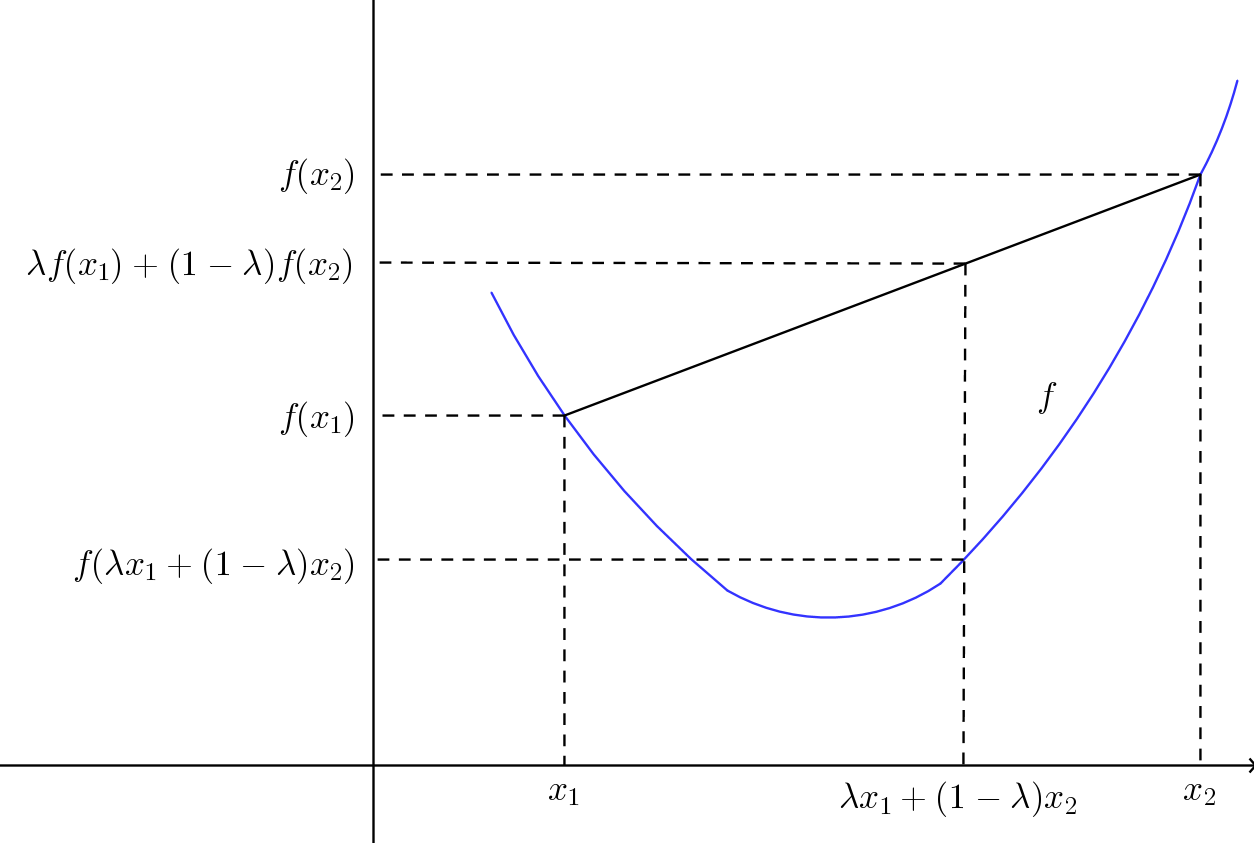
\includegraphics{./partes/sub_sec/codigo-image/f_convx.png}
   \caption{{\footnotesize Interpretaci\'on geom\'etrica de funci\'on convexa en $\mathbb{R}$ \cite{apoyo}}}
   \label{f-convx}
\end{figure}


Los siguientes son algunos ejemplos de funciones convexas.\\

\begin{enumerate}
   \item $f(x) = 3x + 4$
   \item $f(x) = |x|$
   \item $f(x) = x^2 - 2x$
   \item $f(x) =  \displaystyle \left( -x \right)^\frac{1}{2}$
   \item $f(x_1, x_2) = 2x_{1}^2 + 2x_{2}^2 - 2 x_1 x_2$
   \item $f(x_1, x_2, x_3) = x_{1}^{4} + x_{2}^{2} + 3x_{3}^{2} - 4x_1 - 4x_{2} x_{3}$
\end{enumerate}


Note que en cada uno de los ejemplos las funciones son convexas sobre $\mathbb{R}^n$. Excepto para el ejemplo 4, la funci\'on no est\'a
definida para $x < 0.$ Se pueden construir ejemplos de funciones que son convexas en una regi\'on pero no sobre $\mathbb{R}^n$. Por
ejemplo $f(x) = x^3$  no es convexa sobre $\mathbb{R}$, pero es convexa sobre $S= \{x:\, x \geqslant 0\}.$ Un ejemplo de ello es $f(x) = x^3$
no es convexa sobre $\mathbb{R}$ pero lo es sobre $S = \{x: x \geqslant 0\}.$\\ \\

De ahora en adelante nos concentraremos en funciones convexas, pues el resultado para funciones c\'oncavas puede ser obtenido f\'acilmente
notando que $f$ es c\'oncava si y s\'olo si $-f$ es convexa.\\ \\


Un conjunto asociado a una funci\'on convexa $f$ es $S_{\alpha} = \{x \in S: f(x) \leqslant \alpha \}, \,\, \alpha \in \mathbb{R}$, 
usualmente referido como {\it conjunto de nivel}. A veces este conjunto es llamado un {\it conjunto subnivel}, para
diferenciarlo del {\it conjunto supernivel} $\{ x \in S:\,  f(x) \geqslant \alpha \}$ note que \'estos tienen propiedades a 
las de una funci\'on c\'oncava. \\ \medskip

{\teorema Sea $S$ un conjunto convexo no vac\'io en $\mathbb{R}^n$ y sea $f: S \longmapsto \mathbb{R}$ una funci\'on convexa. Entonces el 
conjunto de nivel $S_{\alpha} = \{ x \in S:\, f(x) \leqslant\alpha \}; \,\, \alpha \in \mathbb{R}$ donde es un n\'umero real, es un 
conjunto convexo. \label{nivel-convx} }\\ 

\textbf{\itshape Demostraci\'on:}\\
Sean $x_1, x_2\, \in S_{\alpha}.$ Entonces $x_1, x_2\, \in S$  y  $f(x) \leqslant \alpha$  y  $f(x) = \alpha$. Ahora, sea $\lambda \in (0, 1)$
y $x = \lambda x_1 + (1 - \lambda)x_2$. Por la convexidad de $S$ se tiene que $x \in S$, por otro lado, dada la convexidad de $f$ se tiene:

$$f(x) = \lambda f(x_1) + (1 - \lambda) f(x_2) \leqslant \lambda \alpha (1 - \lambda)\alpha = \alpha$$

Por lo tanto, $x \in S_{\alpha},$ y por consiguiente, $S_{\alpha}$ es convexo.
\begin{flushright}
   $\square$
\end{flushright}

\medskip

\textbf{Continuidad de funciones convexas}\\\\

Una propiedad importante de funciones convexas y c\'oncavas es que son continuas en el interior de su dominio.\\ \\

{\teorema Sea $S$ un conjunto convexo no vac\'io en $\mathbb{R}^n$ y sea $f: S \longmapsto \mathbb{R}^n$ una funci\'on convexa. Entonces $f$
es continua en el interior de $S.$ \label{fconvex-continuos} }\\

%hacer demostracion? esta bastnte larga
% \textbf{\itshape Demostraci\'on:}\\
% Sea $\overline{x} \in \mathring{S}$. Para probar la continuidad de $f$ en $\overline{x}$, es necesario mostrar que dado $\varepsilon > 0$
% existe un $\delta > 0$ tal que $\parallel x - \overline{x} \parallel \leqslant \delta $

Note que las funciones convexas y c\'oncavas pueden no ser continuas en todo lugar. Sin embargo, por el Teorema (\ref{fconvex-continuos}), 
los puntos de discontuindad solo son permitidos en la frontera de $S$, como se ilustra en la siguiente funci\'on convexa definida en 
$S = \{ x:\, -1 \leqslant x \leqslant 1 \}$:

\[f(x) = \displaystyle{\left \{ \begin{array}{lcl}
                                  x^2 &\mbox{para}& |x| < 1\\
                                  2 &\mbox{para}& |x| = 1
                               \end{array}
\right.}\]










